If you are using the Arduino IDE, use \textit{pollinglab-arduino.zip} or \textit{pollinglab-arduino.tar}.
If you are using the VS Code with PlatformIO, use \textit{pollinglab-platformio.zip} or \textit{pollinglab-platformio.tar}.
Download the zip file or tarball from \filesource.
Once you have downloaded the file, close any existing projects in your IDE, unpackage the file, and open the project in your IDE\@.

\textcolor{red}{\textbf{Important}} If you are using the Arduino~IDE, go into the Arduino~IDE's Library Manager to see if you need to update the CowPi library to version 0.6.1.
(PlatformIO on VS~Code will automatically update the library when it reads the project's \textit{platformio.ini} file.)

\begin{figure}[h]
    \centering
    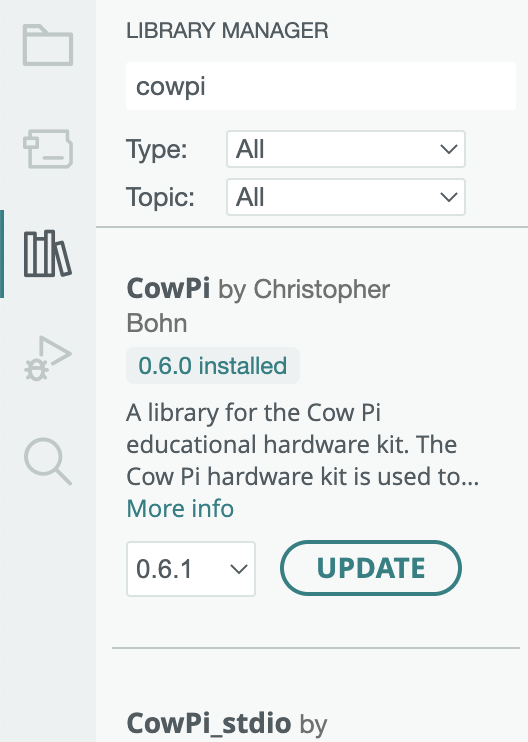
\includegraphics[height=5cm]{libraryUpgrade}
\end{figure}

\vspace{1cm}

Position both of your Cow Pi's switches in the \textit{right} position.
Connect your computer to your Cow Pi and upload the program to your Cow Pi.
The display module will show: \\
\display{
    \colorbox{LightGreen}{KEY\phantom{xxx}BTN\phantom{xxx}SW\phantom{x}} \vspace{-1mm}\\
    \colorbox{LightGreen}{\phantom{x}-\phantom{xxxx}U\phantom{x}U\phantom{xxx}R\phantom{x}R}
} \\
and the right LED (the external LED) will be illuminated.

If you forgot to place the \textbf{left switch} in the \textit{right} position, you will not have that output.
Toggle the left switch to the right and press the RESET button in the middle of the \developmentboard.
This will activate the I/O test code for this lab.

While this I/O test code is running, the display module (and the Serial Monitor) will always show the position of each of the pushbuttons (``U'' = up, ``D'' = down) and each of the switches (``L'' = left position, ``R'' = right position).
The code that determines which key (if any) on the numeric keypad is pressed will work after you write a small amount of code in Section~\ref{subsec:populatekeypad}, which the TAs will guide you through.
\textit{Do not press more than one key on the keypad at the same time.}
If both pushbuttons are pressed, then the left LED (the LED on the \developmentboard) will illuminate,
and if both switches are toggled to the right, then the right LED will illuminate.


\subsection{Description of PollingLab Files}

\subsubsection{PollingLab.ino or PollingLab.cpp}

Do not edit \textit{PollingLab.ino} or \textit{PollingLab.cpp}.

\textit{PollingLab.ino} is in the package for the Arduino IDE, and \textit{PollingLab.cpp} is in the package for PlatformIO.
Whichever you are using, this file contains the code to configure your Cow~Pi for this lab and the code that determines whether to run the I/O test or the simple embedded system that you will write.

%\subsubsection{i2c\_address.h}
%
%This file exists solely to store the display module's I$^2$C address.
%You do not need to edit it further.
%
%\subsubsection{supplement.h}
%
%Do not edit \textit{supplement.h}.
%
%This file contains code that we hope will make it easier for you to focus on this assignment's learning objectives by taking care of a couple of the complexities.
%These functions are not yet in the CowPi library but soon may be, depending on how well they work for you.

\subsubsection{io\_functions.h \& io\_functions.c}

Do not edit \textit{io\_functions.h}.

The \textit{io\_functions.c} file contains functions that you will edit in Sections~\ref{sec:LabTime} and Section~\ref{sec:MemMapIO}.
The functions that read the inputs and write to the outputs currently make use of CowPi library functions.
Your task will be to replace those library calls with code that uses the microcontroller's memory-mapped I/O registers.

\subsubsection{number\_builder.h \& number\_builder.c}

Do not edit \textit{number\_builder.h}.

The \textit{number\_builder.c} file contains a function, \function{build_number()}, that the driver code will call when you are not running the I/O test.
Right now that function is only a stub.
In Section~\ref{sec:SimpleSystem}, you will write code in \function{build_number()} (and in helper functions of your devising) to implement a simple system's specification.


\subsection{Debouncing} \label{subsec:debouncing}

\begin{figure}[h]
    \centering
    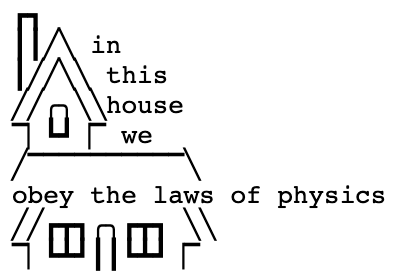
\includegraphics[height=3.5cm]{in-this-house}
\end{figure}

Mechanical buttons and switches demonstrate a phenomenon called \textit{switch bounce}.
This causes voltage to fluctuate for hundreds, often thousands, of microseconds when the contacts close or open.
When this fluctuation is in the indeterminate region between the logical low and high thresholds, it can cause the logic level to ``bounce'' back-and-forth between high and low until settling into the final, correct logic level.
This causes the digital circuitry or software to ``see'' multiple triggering events.

%A traditional way to debounce is to introduce a simple low-pass filter using a resistor and a capacitor.
%Other common hardware-based approaches use digital feedback circuits.

%Hardware design can be simplified by solving a hardware problem with software, and so you will often see hobby projects with ``debouncing code'' such as \lstinline{delay(20);} that pauses execution between detecting the first change of the button's or switch's position and acting upon it for 20ms, which should be ample time for switch bounce to stabilize.
%A problem (beyond \function{delay()} being disallowed in this lab) is that 20ms is a long time to leave your system completely non-responsive.
%
%A better solution is to continue to record the system time when a button is actually pressed or a switch is actually toggled and the device's position after that ``true action.''
%When the button or switch is polled, if fewer than 20ms have passed then ignore the actual device and report the position that resulted from the last true action.
%If more than 20ms have passed then check the device, then report the device's actual position (and also record the system time and the device's position).
%This solution allows your system to continue to respond to other external events.
%For example, you can press both buttons at very nearly the same time (or, unlikely, at the exact same time) and the software will react to both immediately.
%
%The non-blocking solution just described usually works.
%Most switch bounce finishes in under a millisecond.
%Switch bounce almost always finishes in under ten milliseconds.
%Whether using a blocking or non-blocking solution, 20ms should be ample time for a device to stop bouncing.
%We have found that some batches of the pushbuttons, slide-switches, and keypads that are included in the class kit are particularly ``dirty,'' and we have measured switch bounce sometimes lasting longer than 20ms, sometimes upwards of 150ms.
%(This happens very rarely, but often enough that we're confident it wasn't a measurement error.)
%
%The \textit{supplement.h} file includes a \function{debounce_byte()} function that takes a more-elaborate approach of reporting an input device's last ``good value'' until 20ms after the last detected bounce.
%No matter how long the device bounces, the ``time since last bounce'' resets.
%In this manner, we can be sure that bouncing has stabilized before trusting a new value found on the device.
%
%The functions in \textit{io\_functions.c} make use of \function{debounce_byte()}.
%When you modify these functions, as long as you preserve those \function{debounce_byte()} calls, you do not need to worry further about debouncing.

A traditional way to debounce is to introduce a simple low-pass filter using a resistor and a capacitor.
Other common hardware-based approaches use digital feedback circuits.
Hardware design can be simplified, and manufacturing cost can be reduced, by solving a hardware problem with software.
This, of course, transfers the design complexity to the software.

The CowPi library includes a \function{cowpi_debounce_byte()} function that essentially implements a low-pass filter in software.
The functions in \textit{io\_functions.c} make use of \function{cowpi_debounce_byte()}.
When you modify these functions, as long as you preserve those \function{cowpi_debounce_byte()} calls, you do not need to worry further about debouncing.
